\documentclass{standalone}
\usepackage{tikz-network}

\begin{document}
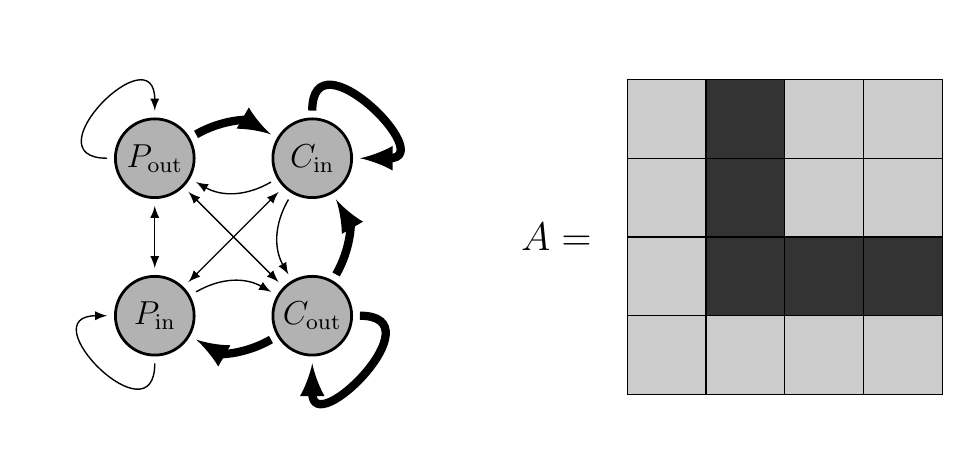
\begin{tikzpicture}

\SetVertexStyle[LineWidth=1, FillColor=black!30!white, LineColor=black, OuterSep=3, TextFont=\large]
\SetEdgeStyle[Color=black]
\SetTextStyle[TextFont=\Large]

\Vertex[label=$P_\mathrm{out}$,size=1]{1}
\Vertex[x=2,label=$C_\mathrm{in}$,size=1]{2}
\Vertex[x=2,y=-2,label=$C_\mathrm{out}$,size=1]{3}
\Vertex[y=-2,label=$P_\mathrm{in}$,size=1]{4}

\Edge[Direct,lw=3,bend=30](1)(2)
\Edge[Direct,lw=3,bend=-30](3)(2)
\Edge[Direct,lw=3,bend=30](3)(4)
\Edge[Direct,lw=3,loopposition=45,loopsize=1cm](2)(2)
\Edge[Direct,lw=3,loopposition=-45,loopsize=1cm](3)(3)
\Edge[Direct,lw=0.5,loopposition=135,loopsize=1cm](1)(1)
\Edge[Direct,lw=0.5,loopposition=-135,loopsize=1cm](4)(4)
\Edge[Direct,lw=0.5,bend=30](2)(1)
\Edge[Direct,lw=0.5,bend=-30](2)(3)
\Edge[Direct,lw=0.5,bend=30](4)(3)
\Edge[Direct,style=latex-latex,lw=0.5](1)(4)
\Edge[Direct,style=latex-latex,lw=0.5](1)(3)
\Edge[Direct,style=latex-latex,lw=0.5](2)(4)

\Text[x=5.1,y=-1]{$A = $}

\draw[fill=black!20!white] (8,0) rectangle ++(1,1);
\draw[fill=black!20!white] (9,0) rectangle ++(1,1);
\draw[fill=black!20!white] (8,-1) rectangle ++(1,1);
\draw[fill=black!20!white] (9,-1) rectangle ++(1,1);
\draw[fill=black!20!white] (6,0) rectangle ++(1,1);
\draw[fill=black!80!white] (7,0) rectangle ++(1,1);
\draw[fill=black!20!white] (6,-1) rectangle ++(1,1);
\draw[fill=black!80!white] (7,-1) rectangle ++(1,1);
\draw[fill=black!20!white] (6,-2) rectangle ++(1,1);
\draw[fill=black!80!white] (7,-2) rectangle ++(1,1);
\draw[fill=black!20!white] (6,-3) rectangle ++(1,1);
\draw[fill=black!20!white] (7,-3) rectangle ++(1,1);
\draw[fill=black!80!white] (8,-2) rectangle ++(1,1);
\draw[fill=black!80!white] (9,-2) rectangle ++(1,1);
\draw[fill=black!20!white] (8,-3) rectangle ++(1,1);
\draw[fill=black!20!white] (9,-3) rectangle ++(1,1);

\end{tikzpicture}
\end{document}